
\section{Kuželosečky}\label{appb}
\subsection*{Označení}
Obecná rovnice kuželosečky:
$$
    \textcolor{magenta}{a_{11}}x^2 + 2 \textcolor{blue}{a_{12}}xy +
    \textcolor{red}{a_{22}}y^2 + 2 \textcolor{gray}{a_{13}}x +
    2 \textcolor{teal}{a_{23}}y + \textcolor{brown}{a_{33}}=0
$$
Matice kuželosečky:
$$
K=\begin{pmatrix}
    \textcolor{magenta}{a_{11}} & \textcolor{blue}{a_{12}} & \textcolor{gray}{a_{13}}\\
    \textcolor{blue}{a_{12}} & \textcolor{red}{a_{22}} & \textcolor{teal}{a_{23}} \\
    \textcolor{gray}{a_{13}} & \textcolor{teal}{a_{23}} &  \textcolor{brown}{a_{33}}
\end{pmatrix}
$$

Diskriminant kuželosečky:
$$
    \Delta = \det K
$$

Diskriminant kvadratických členů (malý diskriminant):
$$
    \delta = \det A = \begin{vmatrix}
        \textcolor{magenta}{a_{11}} & \textcolor{blue}{a_{12}}\\
        \textcolor{blue}{a_{12}} & \textcolor{red}{a_{22}}
    \end{vmatrix}
$$

\subsection*{Regulární kuželosečky}
Platí $\Delta \ne 0.$ (Hodnost matice $K$ je 3.)
\begin{itemize}
\item $h(A)=2$: \textbf{středové} ($\delta \ne 0$):
\begin{center}
    \begin{tabular}{c c c c}
        $\frac{x^2}{a^2}+\frac{y^2}{b^2}=-1$ & imaginární elipsa & $\begin{pmatrix}
            + & 0 & 0 \\
            0 & + & 0 \\
            0 & 0 & 1
        \end{pmatrix}$ & $\delta >0, \Delta >0$ \\[1cm]
        $\frac{x^2}{a^2}+\frac{y^2}{b^2}=1$ & elipsa & $\begin{pmatrix}
            + & 0 & 0 \\
            0 & + & 0 \\
            0 & 0 & -1
        \end{pmatrix}$ & $\delta >0, \Delta <0$ \\[1cm]
        $\frac{x^2}{a^2}-\frac{y^2}{b^2}=1$ & hyperbola & $\begin{pmatrix}
            + & 0 & 0 \\
            0 & - & 0 \\
            0 & 0 & -1
        \end{pmatrix}$ & $\delta <0, \Delta >0$
    \end{tabular}
\end{center}
\item $h(A)=1$: \textbf{nestředové} ($\delta = 0$):
\begin{center}
    \begin{tabular}{c c c c}
        $y^2-2px=0$ & parabola & $\begin{pmatrix}
            0 & 0 & \pm p  \\
            0 & 1 & 0 \\
            \pm p  & 0 & 0 \\
        \end{pmatrix}$ nebo $\begin{pmatrix}
            1 & 0 & 0  \\
            0 & 0 & \pm p \\
            0  & \pm p & 0 \\
        \end{pmatrix}$ & $\delta =0, \Delta <0$
    \end{tabular}
\end{center}
\end{itemize}

\subsection*{Singulární kuželosečky}
Platí $\Delta = 0.$ (Hodnost matice $K$ je menší než 3.)

\begin{itemize}
\item $h(K)=2, h(A)=2$: \textbf{různoběžky} ($\delta \ne 0$):
\begin{center}
    \begin{tabular}{c c c c}
        $x^2-k^2y^2=0$ & dvě různoběžky & $\begin{pmatrix}
            + & 0 & 0 \\
            0 & - & 0 \\
            0 & 0 & 0
        \end{pmatrix}$ & $\delta <0, \Delta =0$ \\[1cm]
        $x^2+k^2y^2=0$ & bod & $\begin{pmatrix}
            + & 0 & 0 \\
            0 & + & 0 \\
            0 & 0 & 0
        \end{pmatrix}$ & $\delta >0, \Delta =0$
    \end{tabular}
\end{center}
\item $h(A)=1$: \textbf{rovnoběžky} ($\delta = 0$):
\begin{center}
    \begin{tabular}{c c c c}
        $x^2-r^2 = 0$ & dvě různé rovnoběžky & $\begin{pmatrix}
            + & 0 & 0  \\
            0 & 0 & 0 \\
            0 & 0 & -
        \end{pmatrix}$ & $\delta =0, \Delta =0$ \\[1cm]
        $x^2+r^2 = 0$ & prázdná množina & $\begin{pmatrix}
            + & 0 & 0  \\
            0 & 0 & 0 \\
            0 & 0 & +
        \end{pmatrix}$ & $\delta =0, \Delta =0$ \\[1cm]
        $x^2 = 0$ & přímka & $\begin{pmatrix}
            + & 0 & 0  \\
            0 & 0 & 0 \\
            0 & 0 & 0
        \end{pmatrix}$ & $\delta =0, \Delta =0$
    \end{tabular}
\end{center}
\end{itemize}

\subsection*{Elipsa}
Množina všech bodů $X$ v rovině, které mají od dvou bodů $F_1, F_2$
(ohnisk) konstantní vzdálenost $2a$:
$$|XF_1| + |XF_2|=2a,$$
přičemž $|F_1F_2|<2a$ (neboli $e<a$).
Zvolíme-li kartézskou soustavu souřadnic tak, aby $F_1 = [-e,0], F_2=[e,0],
X[x,y],$ pak postupnou úpravou dostaneme
$$\frac{x^2}{a^2}+\frac{y^2}{b^2}=1.$$

\begin{minipage}{0.48\linewidth}
\begin{itemize}
\item hlavní, vedlejší vrcholy
\item $F_1, F_2$ ohniska
\item $a$ hlavní poloosa
\item $b$ vedlejší poloosa
\item $c$ (značíme $e$) excentricita, platí $a^2=b^2+e^2$
\item numerická excentricita $\varepsilon = e/a$
\item $C$ (značíme $S$) střed
\end{itemize}
\end{minipage}
\hfill
\begin{minipage}{0.48\linewidth}
    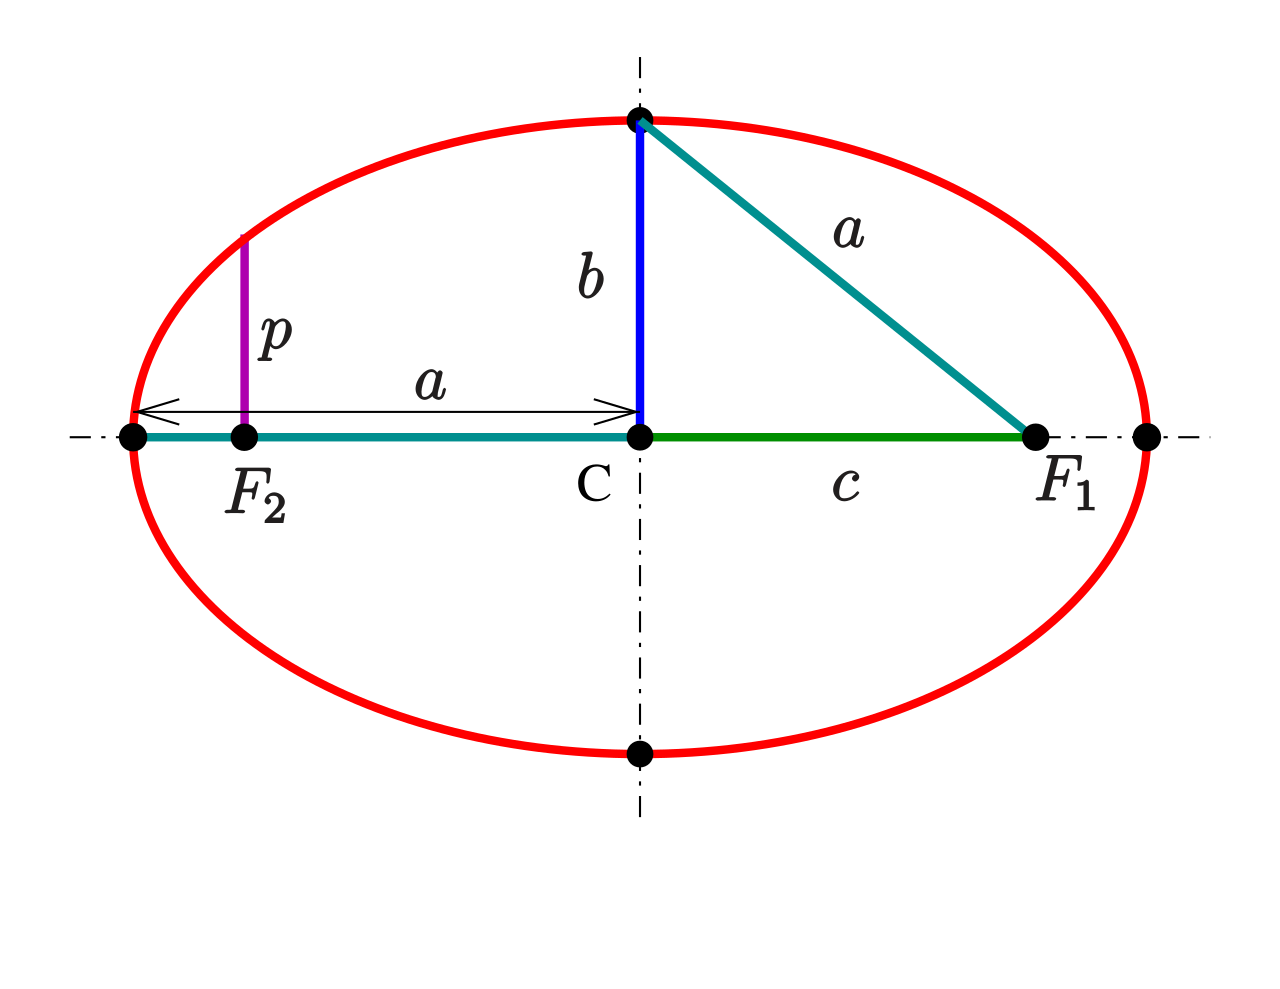
\includegraphics[width=\linewidth]{elipsa.png}
\end{minipage}


\subsection*{Parabola}
Množina všech bodů $X$ v rovině, které mají od přímky $d$ (řídící přímky) a bodu $F$
(ohniska) stejnou vzdálenost:
$$|XF|=|Xd|.$$
Zvolíme-li kartézskou soustavu souřadnic tak, aby $d:x+e=0, F=[e,0],$ pak postupnou
úpravou dostaneme
$$y^2=4ex.$$
Označíme-li vzdálenost ohniska od řídící přímky jako $p=2e,$ dostaneme rovnici tvaru
$$y^2=2px.$$

\begin{minipage}{0.48\linewidth}
\begin{itemize}
\item $V$ vrchol
\item $F$ ohnisko
\item $d$ řídící přímka
\item $p$ parametr
\item $o$ osa
\end{itemize}
\end{minipage}
\hfill
\begin{minipage}{0.40\linewidth}
    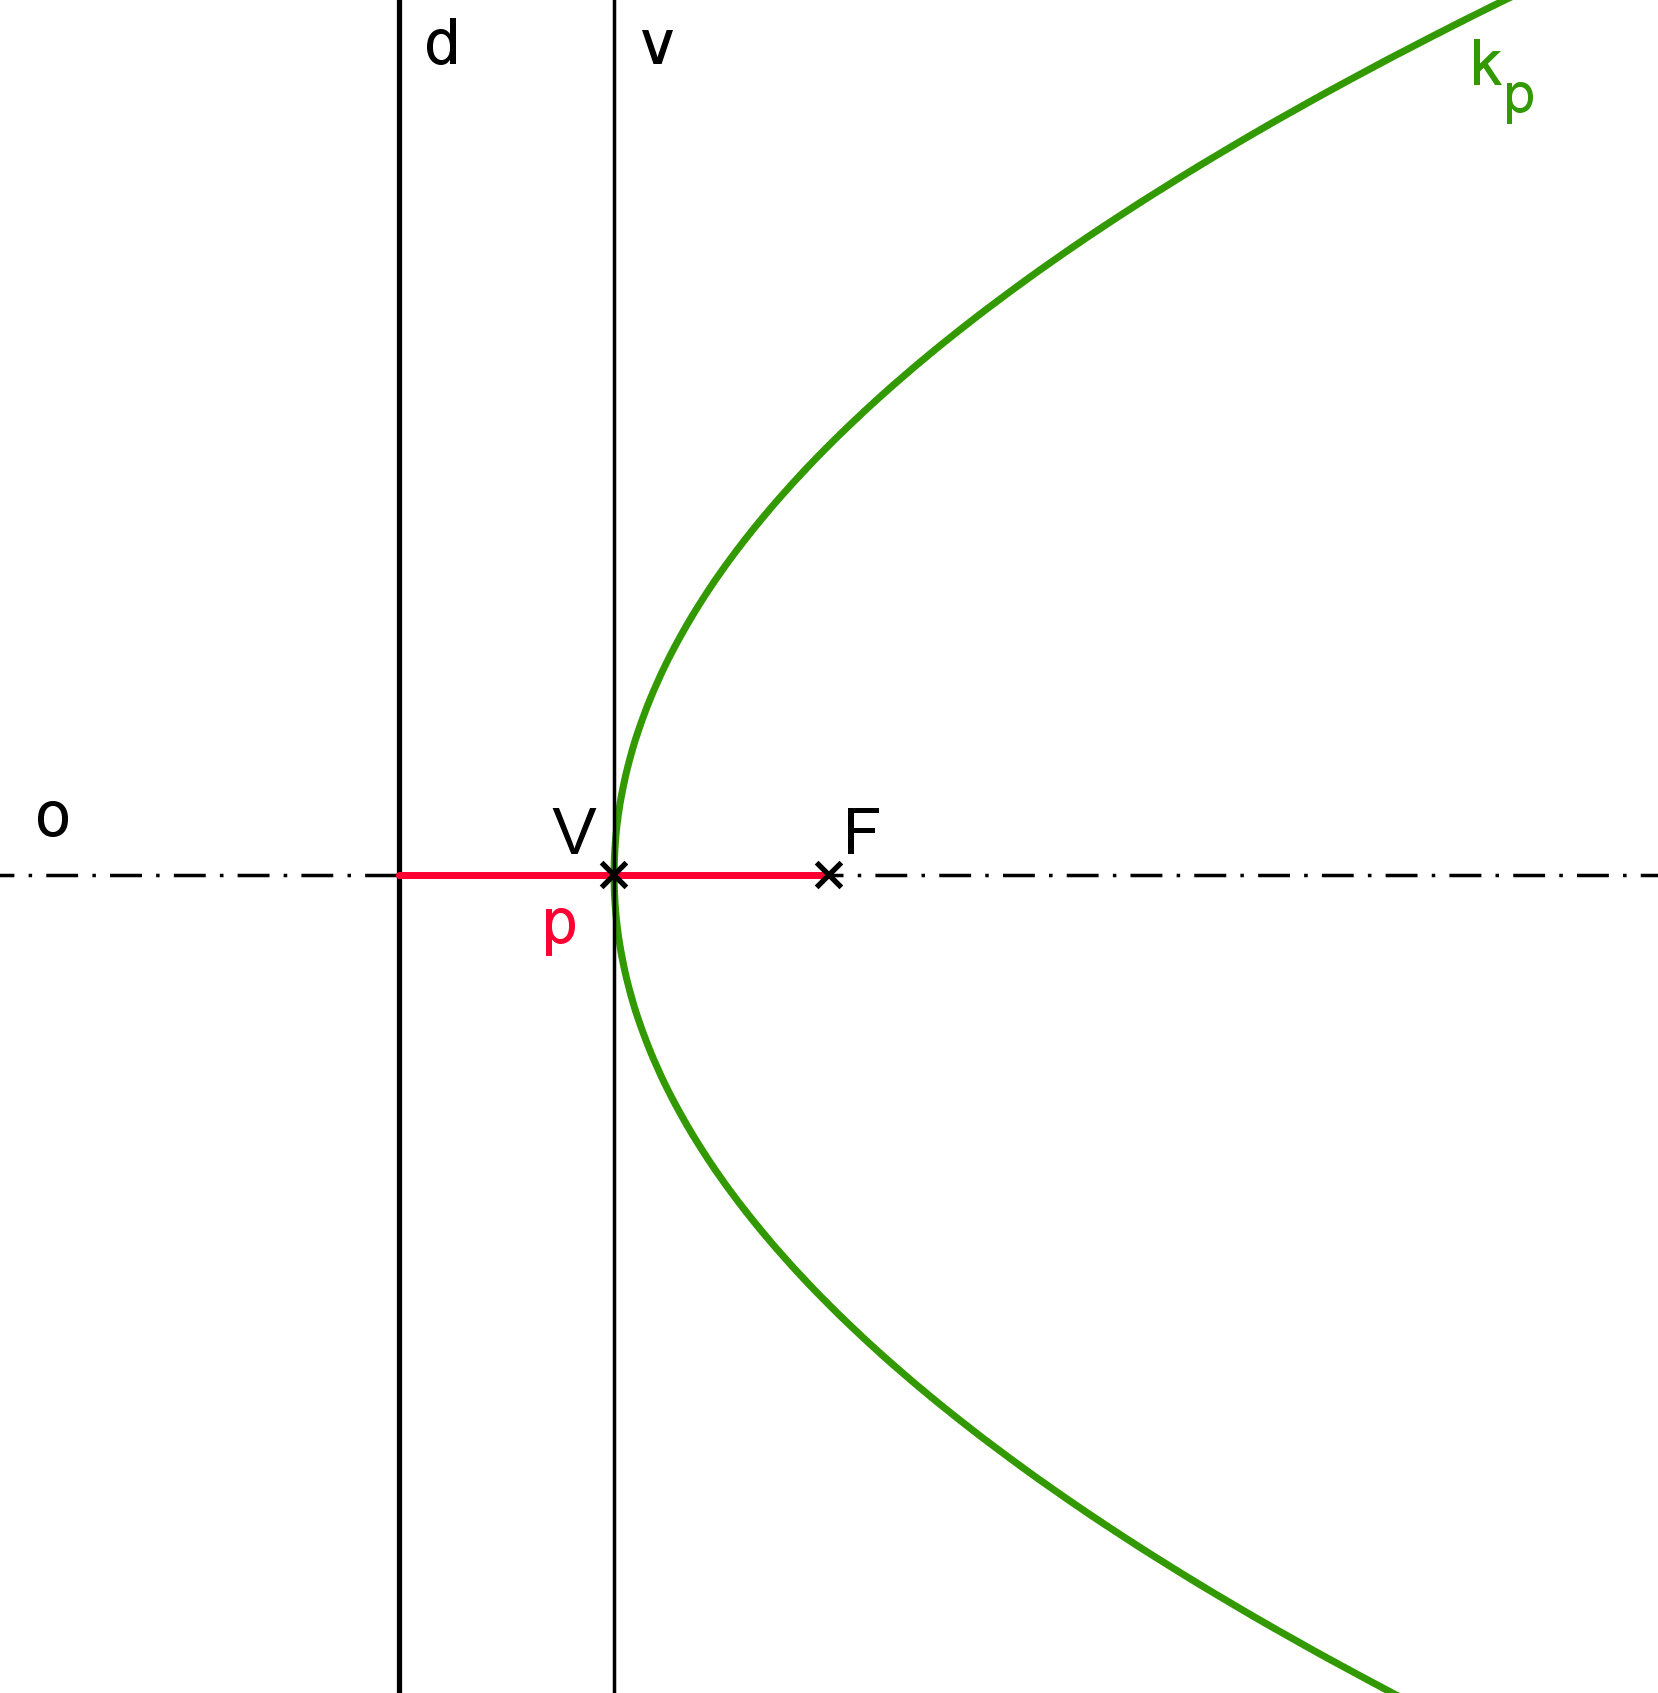
\includegraphics[width=\linewidth]{parabola.png}
\end{minipage}

\begin{pozn}[Rovnice řídící přímky]
    Parabola s vrcholem v bodě $V[m,n]$ má rovnici
    $$x=m-\frac{p}{2}.$$
\end{pozn}

\begin{pozn}
\begin{itemize}
\item $y^2=2px$ -- řídící přímka je rovnoběžná s osou $y$
\item $x^2=2py$ -- řídící přímka je rovnoběžná s osou $x$
\end{itemize}
\end{pozn}

\subsection*{Hyperbola}
Množina všech bodů $X$ v rovině, které mají od dvou bodů $F_1, F_2$
(ohnisk) konstantní absolutní hodnotu rozdílu vzdálenosti $2a$:
$$||F_1X|-|F_2X||=2a.$$
Zvolíme-li kartézskou soustavu souřadnic tak, aby $F_1[-e,0], F_2[e,0],
X[x,y],$ postupnou úpravou dostaneme
$$\frac{x^2}{a^2}-\frac{y^2}{b^2}=1.$$

\begin{minipage}{0.48\linewidth}
\begin{itemize}
\item $S$ střed
\item $F_1,F_2$ ohniska
\item hlavní, vedlejší vrcholy
\item asymptoty
\item $a$ hlavní poloosa
\item $b$ vedlejší poloosa
\item $e$ excentricita, platí $e^2=a^2+b^2$
\end{itemize}
\end{minipage}
\hfill
\begin{minipage}{0.48\linewidth}
    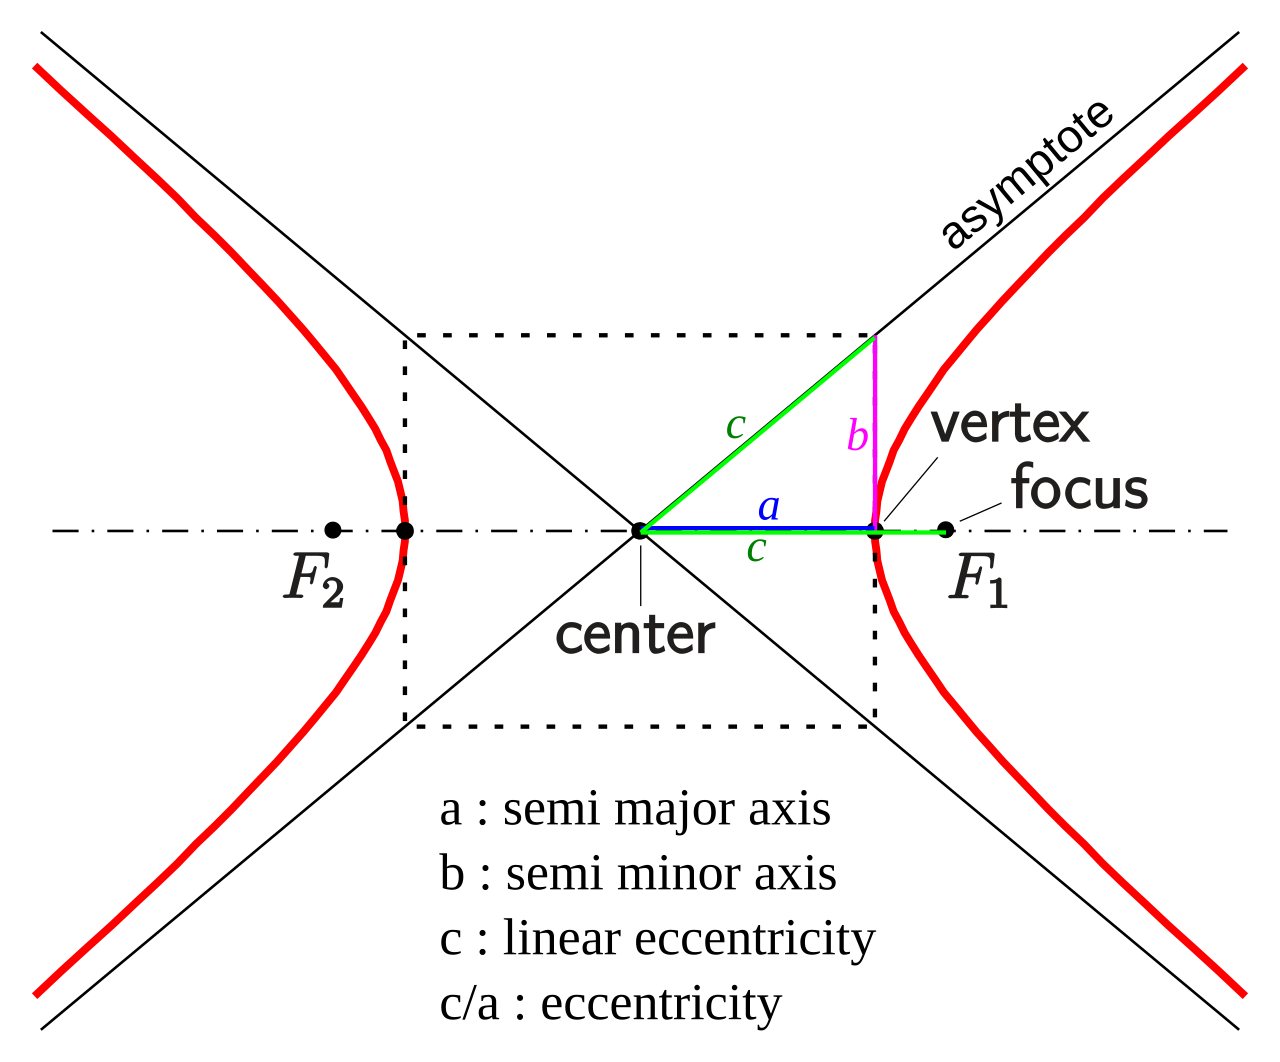
\includegraphics[width=\linewidth]{hyperbola.png}
\end{minipage}
